%%%% 
% This is a template for project reports in the subject DAT620 at the
% Department of Electrical Engineering and Computer Science,
% University of Stavanger.
% 
% The template is based on the ACM conference template 
% it was edited by Leander Jehl and Hein Meling
\documentclass[sigconf]{acmart}\settopmatter{printfolios=true,printccs=false,printacmref=false}
% Set paper size of Report
\geometry{a4paper}

\usepackage{enumitem}
\usepackage{tcolorbox}

\setcopyright{none}
\acmDOI{}
\acmISBN{}
\acmConference{Computational Intelligence Lab}{\today}{Zurich}
\copyrightyear{2021}

%In the preamble file you can include packages and define macros.
\usepackage{xspace}
\usepackage{pdfpages}

%Here we define a marco: The \xspace ensures correct spacing, i.e. insert space before next word, but not before period or comma.
\newcommand{\paxos}{\textsc{Paxos}\xspace}

%These packages are needed for the plot in Figure 1. 
\usepackage{tikz}
\usepackage{pgfplots}
\pgfplotsset{compat=newest}

\def\labelitemi{--}

\usepackage[ruled, linesnumbered]{algorithm2e}
\SetKwProg{Init}{Init:}{}{}

\begin{document}

\title{Reinforced Graph Neural Networks for Collaborative Filtering}

\settopmatter{authorsperrow=4}
\author{Silas Walker}
\affiliation{
	\institution{ETH Zurich, Switzerland}
}
\email{walkers@student.ethz.ch}

\author{Matteo Russo}
\affiliation{
	\institution{ETH Zurich, Switzerland}
}
\email{mrusso@ethz.ch}

\author{Lasse Anthony}
\affiliation{
	\institution{ETH Zurich, Switzerland}
}
\email{laanthony@student.ethz.ch}

\author{Andras Geiszl}
\affiliation{
	\institution{ETH Zurich, Switzerland}
}
\email{ageiszl@student.ethz.ch}

\author{Group: Our Team}


\begin{abstract}
With the rise in popularity of personalized content, smart recommendations are becoming ever more important to get right; they can drive or slash user interaction. One of the most attractive methods to generate predictive compatibility scores for never-before-seen content is collaborative filtering. In this paper, we introduce a collaborative filtering model based on a graph neural network extended with reinforcements and show that this RGNN model can generate user ratings with state-of-the-art accuracy.\footnote{Source code is available at \url{https://github.com/walkersilas/CIL-Project}.}
\end{abstract}

\maketitle

\section{Introduction}
\label{sec:introduction}
Recommendation systems are a core part of many online services today. As more and more content is generated online, providers need a way to decide what content is shown to each of their users to maximize their enjoyment using the service. Recommending the right content can have effect on time spent on the platform as well as improve user experience. 
The popular video streaming service Netflix even introduced an open competition with a grand prize in 2006 for successfully improving on the accuracy of their collaborative filtering model \citep{bennett2007netflix}.

In contract to content-based filtering that uses domain knowledge of users and items such as features of the underlying content and tries to match users with item based on this, collaborative filtering (CF) instead uses the history of the user as well as ratings from other users to predict new ratings. This method can therefore have the advantage of not having to extract features from complex media such as videos or items.

In this work we propose reinforced graph neural networks (RGNNs), a novel approach to tackle the collaborative filtering problem. This approach is based on three core mechanisms: (1) a graph neural network (GNN), (2) a simple feed-forward network, and (3) reinforcements. In particular, the GNN utilizes a bipartite graph built from the user-item rating matrix to gather information between neighboring nodes. This information is then used to generate user and item embeddings which are fed directly into the feed-forward network. The resulting prediction from the feed-forward network and the reinforcements are then used in a final linear layer to obtain the predictions of the RGNN.


\section{Models \& Methods}
\label{sec:models_and_methods}
This section introduces the models and methods used in this work. Firstly, in \autoref{descr} we describe and explore the provided dataset. Secondly, in \autoref{baselines} we outline the baseline approaches used, and finally in \autoref{model} we describe our proposed RGNN architecture.

\subsection{Dataset Description} \label{descr}
The public Kaggle dataset\footnote{Kaggle dataset is available at \url{https://kaggle.com/c/cil-collaborative-filtering-2021/data}.} $X$ used in this work is composed of $|\mathcal{R}| = 1,176,952$ ratings ranging from $1$ to $5$. The ratings are given on $|\mathcal{I}| = 1000$ different items by $|\mathcal{U}| = 10000$ distinct users giving a sparsity of 11.77\% (quotient of total number of entries and observed entries). Compared to the Netflix Prize \citep{bennett2007netflix} and MovieLens \citep{harper2015movielens} datasets, we have a significantly denser data matrix which likely affects the choice of suitable algorithms \citep{lee2012comparative}.

Before proceeding further, we analyze whether matrix completion is information-theoretically possible. Note that most low-rank matrices have a logarithmic strong incoherence property in the order of $\mu^2 \in O(\log n)$ \cite{candestao}. Moreover, given the low sparsity of dataset $X$, we assume that $r = \text{rank}(X) \in O(1)$. By the Candés-Tao theorem \citep{candestao}, we need that the number of observed entries is $\smash{|\mathcal{R}| \in \Omega\left(|\mathcal{U}| \cdot \log^7\left(|\mathcal{U}|\right)\right)}$. Otherwise matrix completion is information-theoretically impossible.
Fortunately, according to the theorem the number of observed entries is sufficient in our case to enable matrix completion.

\subsection{Baselines} \label{baselines}
Our novel model is compared against the following baseline approaches used in collaborative filtering.
\begin{itemize}[leftmargin=0cm]
    \setlength\itemsep{0.6em}
    \item[]
    \textbf{SVD \citep{klema1980singular}:} Singular value decomposition (SVD) is a technique in which the data matrix (supposed all entries are observed) is decomposed into the product of two orthogonal matrices and a central diagonal one. The Eckart-Young theorem \cite{eckart1936approximation} is then used on this decomposition to obtain the best low-dimensional representation of the data. Since the user-item matrix is not complete in our case, the optimization of the recommendation system is done via learning representations of users and items through the alternating least squares (ALS) algorithm or gradient methods. In our implementation SVD uses stochastic gradient descent and is equivalent to probabilistic matrix factorization \citep{sala2007}.
    
    \item[]
    \textbf{SVD++ \citep{koren2008factorization}:} In contrast to SVD, SVD++ takes into account a form of implicit ratings. An implicit rating captures the information that some item is rated by some user. The concrete rating is disregarded in this implicit rating. Similarly to SVD, SGD is used to optimize the SVD++ objective.
    
    \item[]
    \textbf{NMF \citep{zhang2006learning, luo2014efficient}:} Non-negative matrix factorization (NMF) is the problem of approximately factorizing a given matrix by the product of two matrices with non-negative entries. In the context of collaborative filtering, learning such matrices loosely speaking means segmenting the items and users into categories such as genres and preferences. More specifically, the factorization can be interpreted as: (1) How much a user belongs to a certain category, and (2) by which category of users is a certain item preferred.
    
    \item[]\label{sec:slopeone}
    \textbf{SlopeOne \citep{lemire2005slope}:} This algorithm is arguably the simplest form of item-based collaborative filtering. SlopeOne predicts the non-observed rating of a user-item pair solely based on how another similar item has been rated. The prediction is made via a simple linear regressor of slope equal to $1$ (hence, the name) and a bias parameter which is learnt. The simplicity of this model increases computational efficiency. Additionally, overfitting induced by learning the slope vector is reduced.
    
    \item[]
    \textbf{NCF \citep{he2017neural}:} As opposed to canonical matrix factorization approaches, neural collaborative filtering (NCF) replaces the traditional sampling from the inner product between latent codes by a multi-layer perceptron (MLP). Contrary to the proposition in the NCF paper, the generalized matrix factorization (GMF) is omitted in our implementation since the standalone MLP outperformed the combination of the MLP and GMF on our dataset.
    
    \item[]
    \textbf{GNN \citep{wang2019neural}:} The main idea of a graph neural network (GNN) for collaborative filtering consists of representing users and items as nodes of a bipartite graph. Edges between the two partitions of the graph are weighed by a (normalized) rating given by a user for the item. The GNN architecture progressively aggregates and propagates neighborhood latent information generating embeddings of the users and items. Ratings are predicted using a single linear layer. A more detailed description of the GNN and our implementation is provided in \autoref{mapping_and_embedding}.
\end{itemize}


\subsection{Reinforced Graph Neural Networks} \label{model}
We propose the novel architecture: reinforced graph neural networks (RGNNs). The architecture consists of stacking together a graph neural network (as inspired by \citet{wang2019neural, wu2021graph}) with a feed-forward network and adding reinforcements. The graph neural network is the GNN \citep{wang2019neural} and the feed-forward network is the NCF \citep{he2017neural} as described in \autoref{baselines}. The GNN learns the embeddings of users and items, and these embeddings are then pushed through the feed-forward network of the NCF to make reliable and accurate rating predictions. Additionally, we have derived a similar concept to reliabilities introduced by \citet{reliability} which we denote reinforcements (see \autoref{reinforcements}). These concepts allow us to construct a novel architecture obtaining the best of both worlds: (1) The strength of graph-extracted embeddings, and (2) the generalization power of deep learning architectures.

\subsubsection{Theoretical description}
As depicted in \autoref{fig: model}, the RGNN model consists of four phases. The phases can be described disjointly and are: (1) The mapping phase, (2) the embedding phase, (3) the prediction phase, and (4) the combination phase. Note that the phases (1) - (3), described in \autoref{alg:gnn_ncf}, are called GNN + NCF in the remainder of this work. The combination phase (4) predicts a rating from a given output of the GNN + NCF and the corresponding reinforcement. Training the RGNN is done using standard backpropagation minimizing the mean squared error loss.

\begin{figure*}
    \centering
    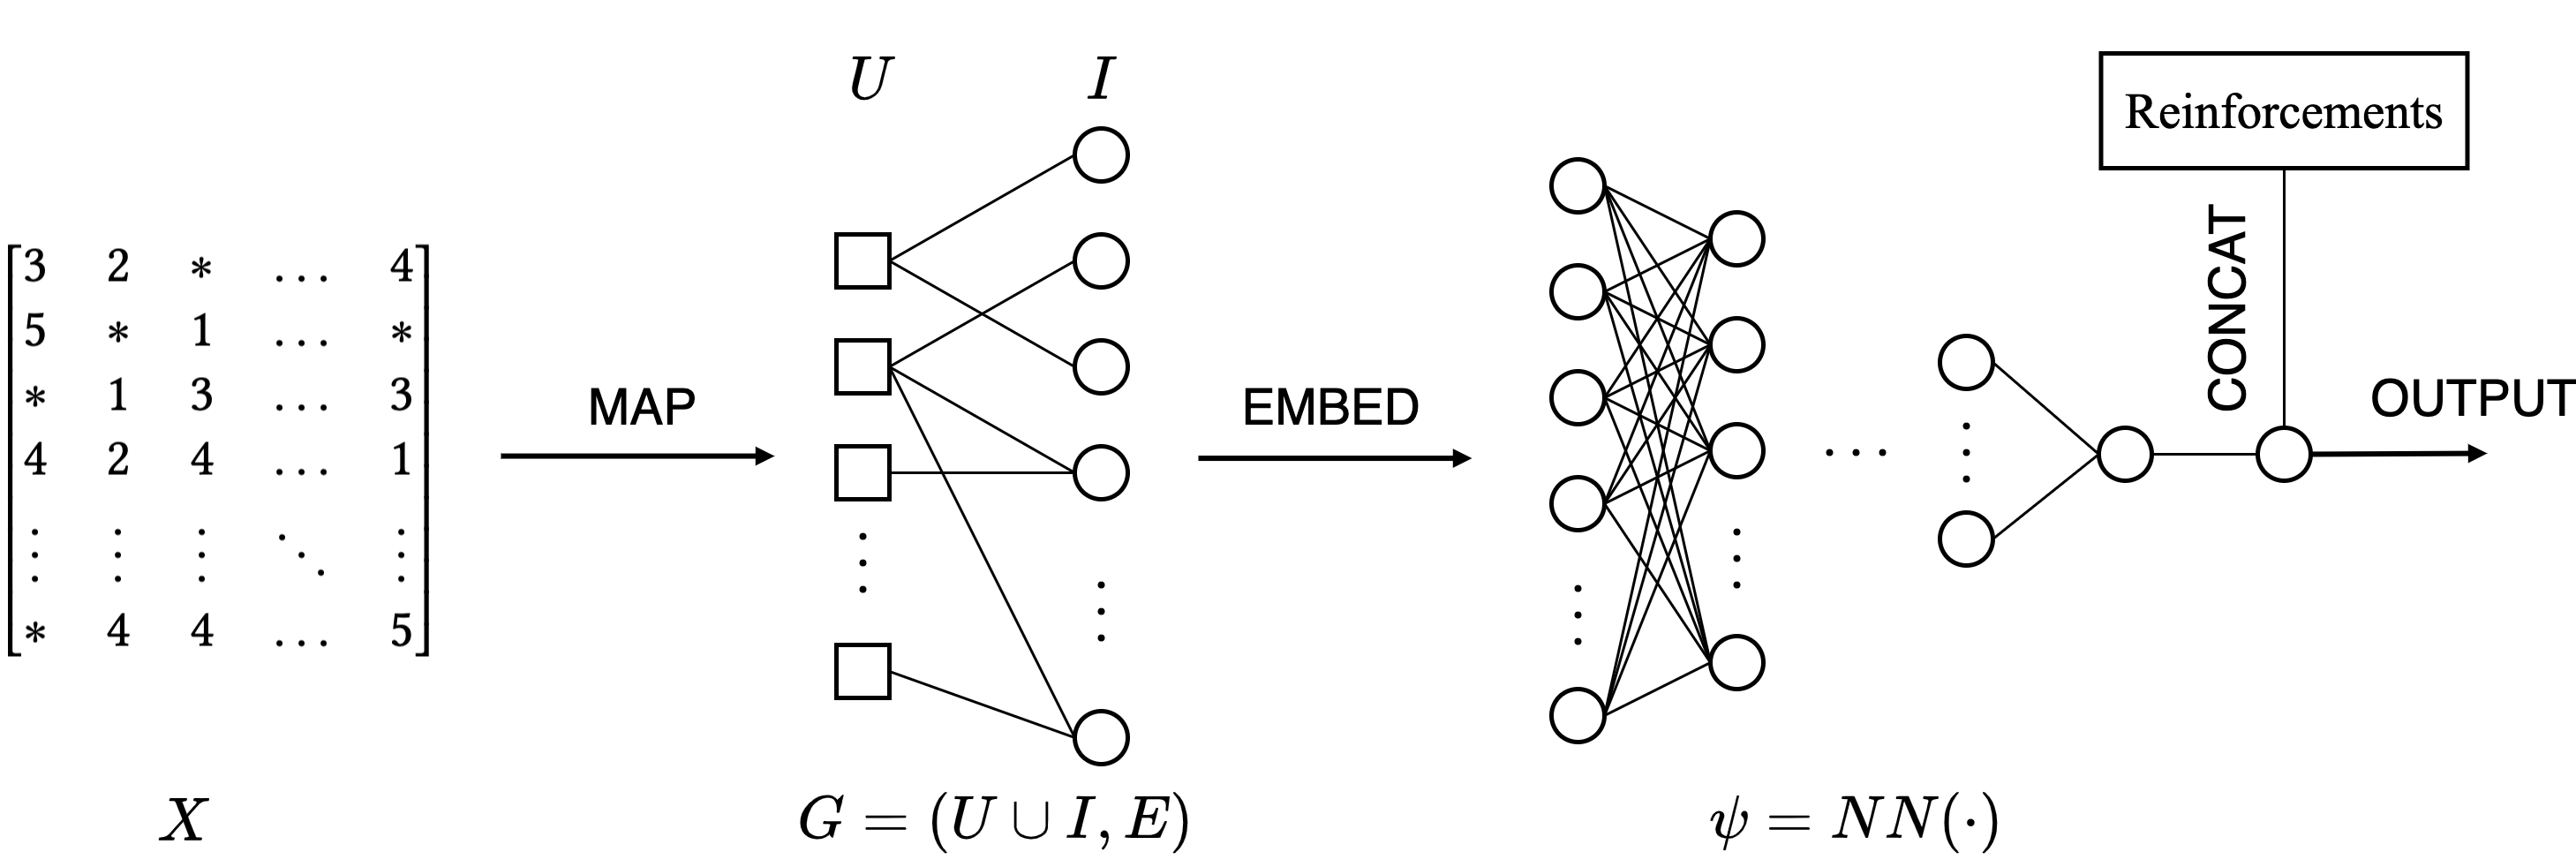
\includegraphics[width=0.9\textwidth]{figures/rgnn_architecture.png}
    \caption{RGNN architecture. (left) Sparse user-item rating data matrix. (center) Bipartite graph representation of the data. (right) Feed-forward neural network that takes the graph-learnt user and item embeddings as well as the reinforcements as input and outputs the rating predictions.}
    \label{fig: model}
\end{figure*}

\subsubsection{Mapping and Embedding}\label{mapping_and_embedding} The dataset $X$ represents the sparse adjacency matrix of the bipartite graph $G = (U \cup I, E)$, where $U$ denotes the partition of user nodes, $I$ the partition of items, and $E$ the set of edges weighted by the observed user-item ratings (line 1 in \autoref{alg:gnn_ncf}). For node $v \in U \cup I$, let $\textbf{m}^{\ell}$ represent the aggregated neighbor information of node $v$ at layer $\ell$, $\textbf{e}^{\ell}_v$ its hidden state (or embedding) at layer $\ell$, and $\textbf{N}_v$ its neighborhood. During the embedding phase, the GNN + NCF algorithm simulates the aggregation of information in the $L$-hop neighborhood of node $v$. This helps extracting higher-order relations between users and items.

The information about nodes in the $L$-hop neighborhood of some node $v \in U \cup I$ is made iteratively and is shown in lines 4 - 7 in \autoref{alg:gnn_ncf}. In particular, at each iteration the aggregated neighbor information $\textbf{m}^{\ell}_v$ of node $v$ is computed by taking the sum over the neighbor information for each neighbor $i \in \textbf{N}_v$ normalized by a discount factor of $\smash{{(\left|\textbf{N}_v\right|\left|\textbf{N}_i\right|})^{-\frac{1}{2}}}$. The discount factor accounts for the decay of the influence of $\ell$-hop neighbors. The neighbor information for a node pair ($v$, $i$) is calculated as a weighted combination of the embedding $\textbf{e}^{\ell}_v$ of node $v$ and the element-wise composition, denoted by $\odot$, of the embedding $\textbf{e}^{\ell}_v$ of $v$ and the embedding $\textbf{e}^{\ell}_i$ of the neighbor $i$. Using the aggregated neighbor information of node $v$ for the $\ell$-hop neighborhood and the $\ell$-hop embedding, we compute the $(\ell + 1)$-hop embedding. This computation takes the sum of the weighted $\ell$-hop embedding and the aggregated neighbor information $\textbf{m}^{\ell}_v$. Further, the Rectified Linear Unit (ReLU) activation function is applied to obtain the $(\ell + 1)$-hop embedding $\textbf{e}^{\ell + 1}_v$. Note that $\textbf{W}_1$ and $\textbf{W}_2$ are the set of parameters that respectively weigh how much the current embedding is influenced by the original features and to what extent the later hops information affects the embedding. An embedding for a node $v$ is then the concatenation of the $\ell$-hop embeddings $\textbf{e}^{\ell}_v$ (line 8 in \autoref{alg:gnn_ncf}).

\subsubsection{Prediction} For a given user-item pair ($u$, $i$), the input to the prediction phase is the embeddings of the user $\textbf{e}^{*}_u$ and item $\textbf{e}^{*}_i$. The output is then computed by the feed-forward network denoted by $\textbf{NN}$ in \autoref{alg:gnn_ncf}. In particular, the feed-forward network is the same as the one used for the NCF baseline (see \autoref{baselines}).

\begin{algorithm}
    \caption{GNN + NCF} \label{alg:gnn_ncf}
    
    \SetAlgoLined
    \DontPrintSemicolon
    \Init{
        Map data matrix $X$ to graph $G = (U \cup I, E)$ \;
    }
    
    \For{$v \in U \cup I$}{
        \For{$\ell \in [L-1]$}{
            $\textbf{m}^{\ell}_v = \sum_{i \in \textbf{N}_v}{\frac{1}{\sqrt{\left|\textbf{N}_v\right|\left|\textbf{N}_i\right|}}\left(\textbf{W}^{\ell}_1\textbf{e}^{\ell}_i + \textbf{W}^{\ell}_2\left(\textbf{e}^{\ell}_i \odot \textbf{e}^{\ell}_v\right)\right)}$ \;
            
            $\textbf{e}^{\ell + 1}_v = \text{ReLU}\left(\textbf{W}^{\ell}_1\textbf{e}^{\ell}_v + \textbf{m}^{\ell}_v\right)$ \;
        }
        
        Concatenate the embeddings: $\textbf{e}^{*}_v = \textbf{e}^{1}_v \oplus \dots \oplus \textbf{e}^{L}_v$ \;
    }
        
    Predict Rating: $\hat{y}(u,i) = \textbf{NN}\left( \textbf{e}^{*}_u\oplus\textbf{e}^{*}_i\right)$ for user-item pair ($u$, $i$) \;
\end{algorithm}

\subsubsection{Reinforcements}\label{reinforcements} Since the input to the GNN + NCF model simply consists of user-item pairs, we aim at providing additional information to the network. Inspired by the approach of \citet{reliability}, where the authors use the prediction accuracy of a model as an additional input to the final model, we introduce reinforcements. Reinforcements consists of predictions from different baseline models. The reinforcements are then fed into a single linear layer together with the output of the GNN + NCF to yield the final predictions of our RGNN. An example of a reinforcement type is the SVD baseline, where the reinforcements for users $u \in U$ and items $i \in I$ are computed using SVD. Then, when introducing the reinforcement for a given user-item pair in the RGNN, the reinforcement intuitively holds the information on how good the SVD baseline prediction is compared to the prediction of the GNN + NCF. This concept is easily extended to different reinforcement types. In particular, our model supports reinforcements from the SVD, SVD++, NMF, and SlopeOne baselines. Additionally, multiple reinforcements can be used simultaneously. However, as we will see in the experimental evaluation of our model in \autoref{sec:results}, the best performance is obtained with a single reinforcement, namely the SlopeOne reinforcement.

\subsubsection{Network Architecture} The RGNN uses two different neural network architectures used for the embedding and predictions. This section provides a brief description of both architectures and the layers used.

The embedding architecture is the GNN baseline and embeds a user or item using three embedding propagation layers. As mentioned in section~\ref{mapping_and_embedding}, these layers accumulate the information in the three-hop neighborhood of the current node in the bipartite graph. The resulting embedding of a user or item is then of size $3 \times 64$.

The prediction architecture is the feed-forward network of the NCF baseline taking as an input the embedding of one user and one item. The network has the following layers: \emph{Dropout, Linear (384), ReLU, Dropout, Linear (64), ReLU, Dropout, Linear (32), ReLU, Linear (16), ReLU, Linear (8), ReLU, Output (1)}. The output of the network is then combined using the reinforcements in a final linear layer. Note that as with the NCF architecture, the prediction architecture contains dropout nodes. However, the optimal dropout rate found during hyperparameter tuning was $0.0$. This supports the findings of the paper introducing graph neural networks \citep{wang2019neural}.

\subsubsection{Ensemble learning}
We improve predictions by utilizing ensembles of our RGNN model with a simple model averaging method for generating the final predictions. We obtained best results using 12 models with SlopeOne reinforcements and different random seeds. We further tried averaging predictions of RGNNs with different reinforcement combinations, however, this showed inferior performance compared to the SlopeOne reinforcements with different random seeds.

\section{Experiments}
\label{sec:results}
\subsection{Experimental Setup}
All experiments were performed on the ETH Leonhard cluster\footnote{\url{https://scicomp.ethz.ch/wiki/Leonhard}} using 1 GPU with 64 GB of RAM and 1 CPU. The simple baselines (SVD, SVD++, NMF, SlopeOne) were developed using Surprise \citep{Hug2020} and the neural network models (NCF, GNN, GNN + NCF, RGNN) were implemented in the PyTorch Lightning framework \citep{falcon2019pytorch} for PyTorch \citep{NEURIPS2019_9015}. The models were trained for a maximum of 60 epochs using the Adam optimizer \citep{kingma2014adam}. We assume model convergence when no improvement in validation loss was observed for 3 consecutive epochs. The model with the lowest validation loss is used as the final model.

As recommended by \citet{rendle2019difficulty}, all baselines are extensively tuned to accurately reflect true model performance. Hyperparameter tuning was done using the Optuna framework \citep{akiba2019optuna} with a sampler using a Tree-Structured Parzen Estimator \citep{bergstra2011algorithms} to suggest parameters for each trial. No pruning was used to stop unpromising trials early; all trials were completed in their entirety. The optimal hyperparameters can be found in the source code. Similarly, extensive neural architecture searches were performed for the NCF and GNN models.

For the RGNN ensemble we further optimize over the random seeds used for each model by choosing the 12 best scoring seeds. We emphasize that this is only done due to the competitive part of the model scoring and the results do not accurately reflect model performance in different environments.

\subsection{Results}
We compare the proposed RGNN model to the various baselines outlined in \autoref{baselines} as well as the GNN + NCF model. We measure model performance with the root mean square error (RMSE) on the public Kaggle dataset. Results from our experiments are summarized in \autoref{tab:results}. We observe that combining the GNN and NCF model into the GNN + NCF model yields a significant performance boost compared to the NCF and GNN baselines. Further improvements can be observed when adding reinforcements to the GNN + NCF model leading to our proposed RGNN model. The training time of the RGNN remains similar to the time of the GNN + NCF model. Employing ensemble learning to the RGNN boosts performance from an RMSE of $0.985$ to $0.982$.

\autoref{tab:results_rgnn} shows model performance by reinforcement used in our RGNN model. Adding reinforcements from the SlopeOne baseline yields the lowest RMSE of $0.9854$. In \autoref{fig:learning_curve_comparison} we further show a comparison of learning curves between our proposed RGNN model and the GNN + NCF baseline. Here we observe that the loss on the held-out validation set fluctuates less through training when reinforcements are used. Since fluctuations in the validation loss are tied to unstable predictions, we conclude that the RGNN makes more stable predictions than the GNN + NCF.

\begin{table}[]
\centering
\begin{tabular}{llr}
\hline
Method & \multicolumn{1}{l}{RMSE} & \multicolumn{1}{l}{Training time (m)} \\ \hline
NCF & $	1.024$ & $65$ \\
SVD & $1.003$ & \boldmath$2$ \\
NMF & $1.000$ & $3$ \\
GNN & $1.000$ & $9$ \\
SVD++ & $0.999$ & $185$ \\
SlopeOne & $0.998$ & $4$ \\
GNN + NCF & $0.988$ & $29$ \\
RGNN & $0.985$ & $26$ \\ 
RGNN ensemble & \boldmath$0.982$ & $437$ \\ \hline
\end{tabular}
\caption{Comparison between various baselines and our proposed RGNN method evaluated on the public Kaggle dataset.}
\label{tab:results}
\end{table}

\begin{table}[]
\centering
\begin{tabular}{ll}
\hline
Reinforcements & RMSE \\ \hline
SVD, NMF & $0.9880$ \\
SVD & $0.9875$ \\
SVD, SVD++ & $0.9875$ \\
SVD, NMF, SlopeOne & \multicolumn{1}{r}{$0.9870$} \\
SVD, SlopeOne & $0.9870$ \\
NMF, SlopeOne & \multicolumn{1}{r}{$0.9870$} \\
SlopeOne, SVD++ & \multicolumn{1}{r}{$0.9869$} \\
SVD, NMF, SVD++ & $0.9868$ \\
NMF & \multicolumn{1}{r}{$0.9868$} \\
NMF, SlopeOne, SVD++ & \multicolumn{1}{r}{$0.9864$} \\
SVD, SlopeOne, SVD++ & $0.9864$ \\
SVD++ & $0.9862$ \\
NMF, SVD++ & \multicolumn{1}{r}{$0.9861$} \\
SVD, NMF, SlopeOne, SVD++ & \multicolumn{1}{r}{$0.9859$} \\
SlopeOne & \multicolumn{1}{r}{\boldmath$0.9854$} \\  \hline
\end{tabular}
\caption{Comparison between reinforcements used in our RGNN model evaluated on the public Kaggle dataset.}
\label{tab:results_rgnn}
\end{table}

\begin{figure}
    \centering
    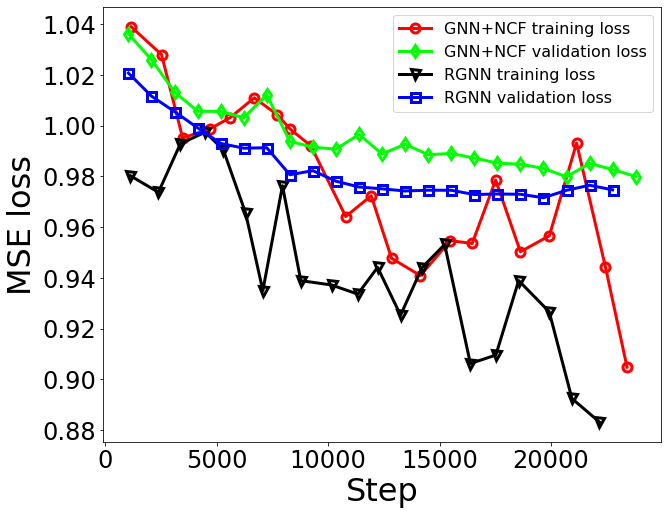
\includegraphics[width=0.45\textwidth]{figures/learning_curve.png}
    \caption{Comparison of learning curves between our RGNN model and the GNN + NCF baseline.}
    \label{fig:learning_curve_comparison}
\end{figure}

\section{Discussion}
\label{sec:discussion}
From \autoref{tab:results} we can observe that RGNN performs significantly better than its baseline counterparts. Models combining graph-extracted information with a feed-forward network, i.e. GNN + NCF and RGNN, perform best in our experiments. This suggests that high-order graph information accurately describes collaborative filtering interactions. Further, we observe that reinforcements improve the performance of the GNN + NCF model. This may be due to the additional information contained in the reinforcements and the final linear layer learning when and how well the user-item pair is representable in the GNN + NCF compared to that of the simple baseline used to generate the reinforcements. As a word of caution: The previous statement is true only when high quality reinforcements are added to the model. Whenever low quality reinforcements, such as those generated by the SVD baseline, are added, the model may overfit to the reinforcements and perform worse (see \autoref{tab:results_rgnn}).

\autoref{tab:results} reports the computation time to run the entire training and prediction process from start to finish. We observe that the neural network models and the SVD++ baseline have the highest time complexity. This may be caused by the neural networks having the largest number of trainable parameters. Conversely, the SVD++ baseline is slow due to not utilizing any fast specialized hardware acceleration such as GPUs. Further, we observe that learning graph embeddings reduces convergence time compared to the standard embeddings in the NCF model.

As already shown by some recent work of Rendle et al. \cite{rendle2019difficulty}, well tuned baselines perform comparably to deep learning models using much less time and resources during the training process. This is also corroborated by our results (see \autoref{tab:results}). The widespread availability of specialized hardware accelerators such as graphics processing units (GPUs) or tensor processing units (TPUs), however, provides wide access to training deep learning architectures with ease like the RGNN proposed in this paper to achieve better performance at the cost of additional training time and resources.

\section{Summary and Future Work}
\label{sec:summary}
In this paper, we develop a graph neural network architecture with added reinforcements from simple matrix factorization techniques for collaborative filtering. This method improves upon several baseline approaches by a significant margin on the public Kaggle dataset (\autoref{tab:results}). 
Following our ablation study comparing the NCF, GNN, and GNN + NCF baselines, we find that model performance depends on both generating meaningful embeddings of users and items and the expressiveness of the neural network used.
We further show that reinforcements generated by the SlopeOne algorithm \citep{lemire2005slope} yields the best results.

In future work, we would like to further explore different types of reinforcements, particularly outputs from more complex models such as neural networks. Similarly, recursive reinforcements can be explored. Extending our experiments to include datasets with a lower sparsity level such as MovieLens can also further investigate the generalizability of our proposed RGNN architecture.



\bibliographystyle{ACM-Reference-Format}
\bibliography{bibliography}

\clearpage

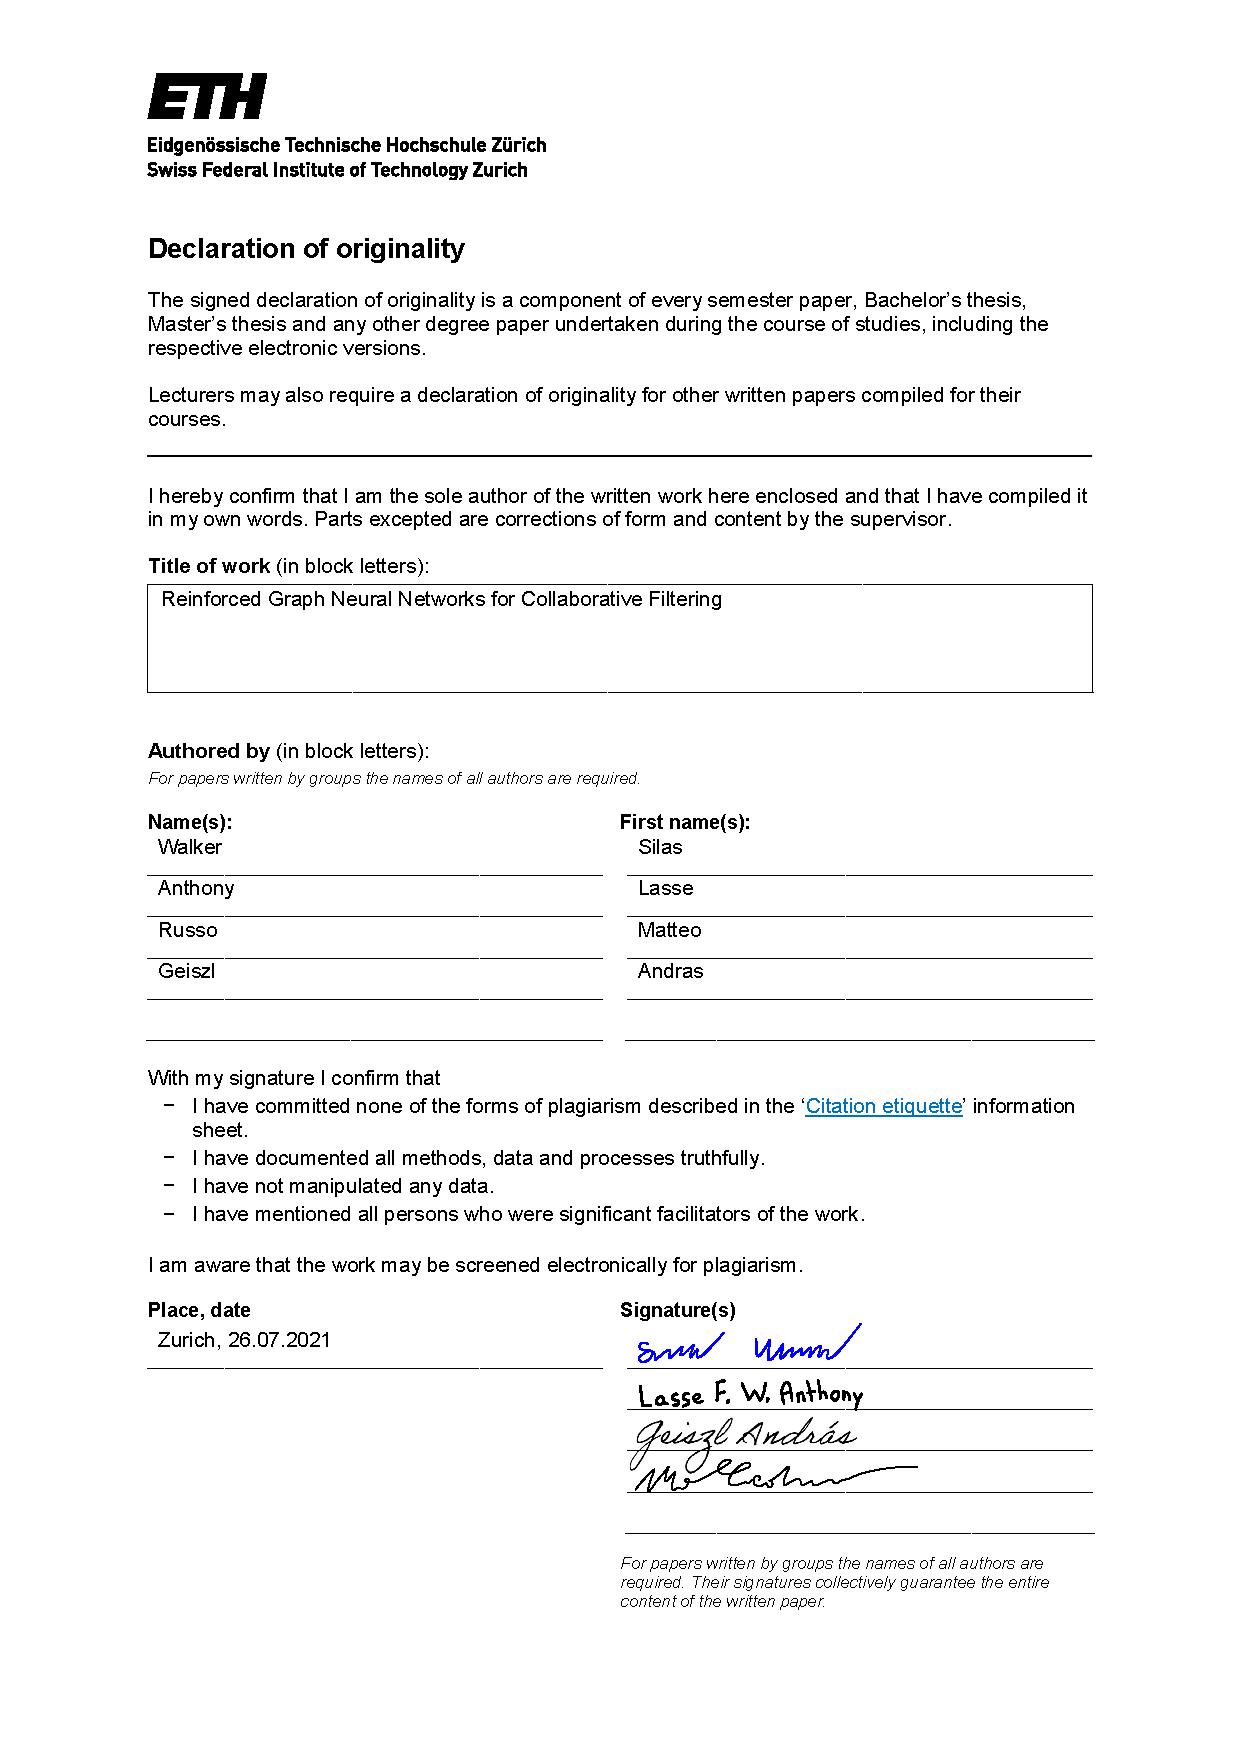
\includepdf[pages=-]{declaration-originality.pdf}

\end{document}
